\documentclass[letterpaper, 11pt]{report}
\usepackage[utf8]{inputenc}
\usepackage{titlesec}
\usepackage{fullpage} % changes the margin
\usepackage{graphicx} %package to manage images
\graphicspath{ {./images/} }

\begin{document}
\begin{titlepage}
\vspace*{0.7in}
\begin{center}
\begin{figure}[htb]
\begin{center}

\includegraphics[width=8cm]{univ_logo}
\end{center}
\end{figure}
\vspace*{0.3in}
\begin{Large}
\textbf{SOEN 6011 : SOFTWARE ENGINEERING PROCESSES} \\
\end{Large}
\vspace*{0.1in}
\begin{Large}
\textbf{SUMMER 2021} \\
\end{Large}
\vspace*{0.9in}
\begin{Large}
\textbf{SUPER CALCULATOR} \\
\end{Large}
\vspace*{0.9in}
\begin{Large} 


\textbf{PROBLEM - 6} \\
Unit Test Cases\\
\end{Large}
\vspace*{0.625in}
\rule{80mm}{0.1mm}\\
\vspace*{0.1in}
\begin{large}
Authors \\
\vspace*{0.1in}
Rokeya Begum Keya\\
\vspace*{0.1in}
Kyle Taylor Lange\\
\vspace*{0.1in}
Sijie Min\\
\vspace*{0.1in}
Manimaran Palani\\ 
\vspace*{0.3in}
\date{\normalsize\today} 
\end{large}
\end{center}
\begin{center}
https://www.overleaf.com/project/610304de4e6b8d24f7c781b6\end{center}
\end{titlepage}
\tableofcontents
\newpage
\addcontentsline{toc}{section}{a) Description on Unit Test Cases }
\newpage
\pagebreak
\section*{Unit Test Cases Description}
\section*{\centering{PROBLEM 6 - F2: $tan(x)$}}
\normalsize {SOEN 6011 - Summer 2021} \hfill \textbf{Rokeya Begum Keya} \\
\textbf{ Software Engineering Processes}  \hfill \textbf{40183615} \\
\hfill Repository address : https://github.com/Dakatsu/SOEN6011Calculator
\\\\\\
\section*{Unit Test Case for F2 Function}
The unit test cases for $tan(x)$ function is done using \textbf{JUnit 4} which are traceable to the requirements in problem-2.\\\\\\
\textbf{Test Case : F2\_UnitTestCase\_1}\\\\
\begin{tabular}{ll}
\textbf{Test Case ID} & F2\_tanZeroCheck\_1\\
\textbf{Requirement ID} & F2-R1 \\
\textbf{Action} & 
\begin{tabular}[c]{@{}l@{}}The user clicks the button "Tan" and gives an input 0 (degree) and
\\then click result(=) button. \\
\end{tabular} \\
\textbf{Input(s) } & $tan(0)$ \\
\textbf{Expected Output } & 0 \\
\textbf{Actual Output } &   0 \\
\textbf{Test Result } & Success \\
\end{tabular}
\\\\\\\\
\textbf{Test Case : F2\_UnitTestCase\_2}\\\\
\begin{tabular}{ll}
\textbf{Test Case ID} & F2\_tanFortyCheck\_2\\
\textbf{Requirement ID} & F2-R2 \\
\textbf{Action} & 
\begin{tabular}[c]{@{}l@{}}The user clicks the button "Tan" and gives an input 40 (degree) and
\\then click result(=) button. \\
\end{tabular} \\
\textbf{Input(s) } & $tan(40)$ \\
\textbf{Expected Output } & 0.83910101 \\
\textbf{Actual Output } & 0.83910101 \\
\textbf{Test Result } & Success \\
\end{tabular}
\\\\\\\\\\\\\\\\\\\\\
\textbf{Test Case : F2\_UnitTestCase\_3}\\\\
\begin{tabular}{ll}
\textbf{Test Case ID} & F2\_tanNinetyCheck\_3\\
\textbf{Requirement ID} & F2-R3 \\
\textbf{Action} & 
\begin{tabular}[c]{@{}l@{}}The user clicks the button "Tan" and gives an input 90 (degree) and
\\then click result(=) button. \\
\end{tabular} \\
\textbf{Input(s) } & $tan(90)$ \\
\textbf{Expected Output } & undefined \\
\textbf{Actual Output } &
undefined \\
\textbf{Test Result } & Success \\
\end{tabular}
\\\\\\\\
\textbf{Test Case : F2\_UnitTestCase\_4}\\\\
\begin{tabular}{ll}
\textbf{Test Case ID} & F2\_tanNegativeValueCheck\_4\\
\textbf{Requirement ID} & F2-R4 \\
\textbf{Action} & 
\begin{tabular}[c]{@{}l@{}}The user clicks the button "Tan" and gives an input 95 (degree) and
\\then click result(=) button. \\
\end{tabular} \\
\textbf{Input(s) } & $tan(95)$ \\
\textbf{Expected Output } & -11.43005230 \\
\textbf{Actual Output } &
-11.43005230 \\
\textbf{Test Result } & Success \\
\end{tabular}
\\\\\\\\
\textbf{Test Case : F2\_UnitTestCase\_5}\\\\
\begin{tabular}{ll}
\textbf{Test Case ID} & F2\_tanNegativeNumberCheck\_5 \\
\textbf{Requirement ID} & F2-R5 \\
\textbf{Action} & 
\begin{tabular}[c]{@{}l@{}}The user clicks the button "Tan" and gives an input -10 (degree) and
\\then click result(=) button. \\
\end{tabular} \\
\textbf{Input(s) } & $tan(-10)$ \\
\textbf{Expected Output } & -0.17723233 \\
\textbf{Actual Output } &
-0.17723233 \\
\textbf{Test Result } & Success \\
\end{tabular}
\\\\\\\\\\\\\\\\\\\\\\\
\textbf{Test Case : F2\_UnitTestCase\_6}\\\\
\begin{tabular}{ll}
\textbf{Test Case ID} & F2\_tanOneHundredAndEightyCheck\_6 \\
\textbf{Requirement ID} & F2-R6 \\
\textbf{Action} & 
\begin{tabular}[c]{@{}l@{}}The user clicks the button "Tan" and gives an input 180 (degree) and
\\then click result(=) button. \\
\end{tabular} \\
\textbf{Input(s) } & $tan(180)$ \\
\textbf{Expected Output } & 0 \\
\textbf{Actual Output } &   0 \\
\textbf{Test Result } & Success \\
\end{tabular}
\\\\\\\\
\textbf{Test Case : F2\_UnitTestCase\_7}\\\\
\begin{tabular}{ll}
\textbf{Test Case ID} & F2\_getRadCheck\_7 \\
\textbf{Requirement ID} & F2-R7 \\
\textbf{Action} & 
\begin{tabular}[c]{@{}l@{}}To make sure that radian function in $tan(x)$ is working properly,
\\I had to do the unit test of Rad(x) and gives an input for $x$ = 90 (degree).
\end{tabular} \\
\textbf{Input(s) } & $Rad(90)$ \\
\textbf{Expected Output } & 1.57079633 \\
\textbf{Actual Output } & 1.57079633 \\
\textbf{Test Result } & Success \\
\end{tabular}
\\\\\\\\
\textbf{Test Case : F2\_UnitTestCase\_8}\\\\
\begin{tabular}{ll}
\textbf{Test Case ID} & F2\_getRadOneHundredAndEightyCheck\_8\\
\textbf{Requirement ID} & F2-R8 \\
\textbf{Action} & 
\begin{tabular}[c]{@{}l@{}}To make sure that radian function in $tan(x)$ is working properly,
\\I had to do the unit test of Rad(x) and gives an input for $x$ = 180 (degree).
\end{tabular} \\
\textbf{Input(s) } & $Rad(180)$ \\
\textbf{Expected Output } & 3.14159 \\
\textbf{Actual Output } & 3.14159 \\
\textbf{Test Result } & Success \\
\end{tabular}
\\\\\\\\\\\\\\\\\\\\\\\\\\\
\textbf{Test Case : F2\_UnitTestCase\_9}\\\\
\begin{tabular}{ll}
\textbf{Test Case ID} & F2\_getSinZeroCheck\_9 \\
\textbf{Requirement ID} & F2-R9 \\
\textbf{Action} & 
\begin{tabular}[c]{@{}l@{}}To make sure that $sin(x)$ function for $tan(x)$ is working properly,
\\I had to do the unit test of $sin(x)$ function and gives an input for 0 (degree).
\end{tabular} \\
\textbf{Input(s) } & $sin(0)$ \\
\textbf{Expected Output } & 0.0 \\
\textbf{Actual Output } &   0.0 \\
\textbf{Test Result } & Success \\
\end{tabular}
\\\\\\\\
\textbf{Test Case : F2\_UnitTestCase\_10}\\\\
\begin{tabular}{ll}
\textbf{Test Case ID} & F2\_getSinFortyCheck\_10\\
\textbf{Requirement ID} & F2-R10 \\
\textbf{Action} & 
\begin{tabular}[c]{@{}l@{}}To make sure that $sin(x)$ function for $tan(x)$ is working properly,
\\I had to do the unit test of $sin(x)$ function and gives an input for 40 (degree).
\end{tabular} \\
\textbf{Input(s) } & $sin(40)$ \\
\textbf{Expected Output } & 0.642788 \\
\textbf{Actual Output } & 0.642788 \\
\textbf{Test Result } & Success \\
\end{tabular}
\\\\\\\\
\textbf{Test Case : F2\_UnitTestCase\_11}\\\\
\begin{tabular}{ll}
\textbf{Test Case ID} & F2\_getCosZeroCheck\_11\\
\textbf{Requirement ID} & F2-R11 \\
\textbf{Action} & 
\begin{tabular}[c]{@{}l@{}}To make sure that $cos(x)$ function for $tan(x)$ is working properly,
\\I had to do the unit test of $cos(x)$ function and gives an input for 0 (degree).
\end{tabular} \\
\textbf{Input(s) } & $cos(0)$ \\
\textbf{Expected Output } & 1 \\
\textbf{Actual Output } &   1 \\
\textbf{Test Result } & Success \\
         \end{tabular}
\\\\\\\\\\\\\\\\\\\\\\\\\\\\\
\textbf{Test Case : F2\_UnitTestCase\_12}\\\\
\begin{tabular}{ll}
\textbf{Test Case ID} & F2\_getCosFortyCheck\_12\\
\textbf{Requirement ID} & F2-R12 \\
\textbf{Action} & 
\begin{tabular}[c]{@{}l@{}}To make sure that $cos(x)$ function for $tan(x)$ is working properly,
\\I had to do the unit test of $cos(x)$ function and gives an input for 40 (degree).
\end{tabular} \\
\textbf{Input(s) } & $cos(40)$ \\
\textbf{Expected Output } & 0.76604305 \\
\textbf{Actual Output } & 0.76604305 \\
\textbf{Test Result } & Success \\
\end{tabular}
\\\\\\\\\
\begin{center}
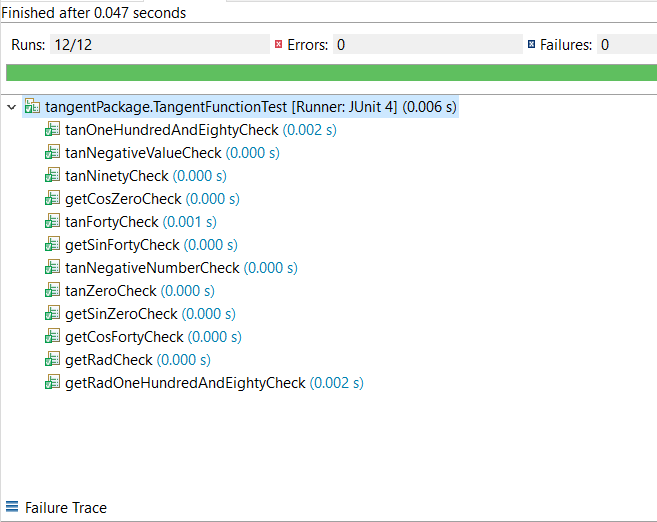
\includegraphics[width= 10cm]{UnitTestCaseF2}
  \begin{center}
Figure: Unit Testing results for tangent function $ (tan(x))$\end{center}
\end{center}
\\\\\\\\

\pagebreak

\section*{\centering{PROBLEM 6 - F3: Hyperbolic Sine, $sinh(x)$}}
\normalsize {SOEN 6011 - Summer 2021} \hfill \textbf{Kyle Taylor Lange} \\
\textbf{ Software Engineering Processes}  \hfill \textbf{27627696} \\https://www.overleaf.com/project/610304de4e6b8d24f7c781b6
\hfill Repository address : https://github.com/Dakatsu/SOEN6011Calculator
\\\\\\

\pagebreak

\section*{\centering{PROBLEM 6 - F5}}
\normalsize {SOEN 6011 - Summer 2021} \hfill \textbf{Sijie Min} \\
\textbf{ Software Engineering Processes}  \hfill \textbf{401*****} \\
\hfill Repository address : https://github.com/Dakatsu/SOEN6011Calculator
\\\\\\\\\\
 \begin{center} Team please add your content here \end{center}
\pagebreak

\section*{\centering{PROBLEM 6 - F7 : \(x^y\)}}
\normalsize {SOEN 6011 - Summer 2021} \hfill \textbf{Manimaran Palani} \\
\textbf{ Software Engineering Processes}  \hfill \textbf{40167543} \\
\hfill Repository address : https://github.com/Dakatsu/SOEN6011Calculator
\\
\section*{\textbf{Problem 6 - Unit Test Case Description}}
This section presents the unit test cases implemented using \textbf{JUnit4} for Super Calculator \\(F7-Power Function) which are traceable to requirements.\\\\\\
\textbf{Test Case : F7\_TestCase\_1}\\\\
\begin{tabular}{ll}
\textbf{Test Case ID} & F7\_TestCase\_1 \\
\textbf{Requirement ID} & F7-R1 \\
\textbf{Action} & 
\begin{tabular}[c]{@{}l@{}}The user inputs a base input and click power function button followed \\by giving exponent input and click result(=) button. \\
\end{tabular} \\
\textbf{Input(s) } & base = 0.0, exponent = 0.0 \\
\textbf{Expected Output } & 1.0 \\
\textbf{Actual Output } & 1.0 \\
\textbf{Test Result } & Success \\
\end{tabular}
\\\\\\\\
\textbf{Test Case : F7\_TestCase\_2}\\\\
\begin{tabular}{ll}
\textbf{Test Case ID} & F7\_TestCase\_2 \\
\textbf{Requirement ID} & F7-R2 \\
\textbf{Action} & 
\begin{tabular}[c]{@{}l@{}}The user inputs a base input and click power function button followed \\by giving exponent input and click result(=) button. \\
\end{tabular} \\
\textbf{Input(s) } & base = 0.0, exponent = 3.0 \\
\textbf{Expected Output } & 0.0 \\
\textbf{Actual Output } & 0.0 \\
\textbf{Test Result } & Success \\
\end{tabular}
\\\\\\\\
\textbf{Test Case : F7\_TestCase\_3}\\\\
\begin{tabular}{ll}
\textbf{Test Case ID} & F7\_TestCase\_3 \\
\textbf{Requirement ID} & F7-R3 \\
\textbf{Action} & 
\begin{tabular}[c]{@{}l@{}}The user inputs a base input and click power function button followed \\by giving exponent input and click result(=) button. \\
\end{tabular} \\
\textbf{Input(s) } & base = 7.0, exponent = 0.0 \\
\textbf{Expected Output } & 1.0 \\
\textbf{Actual Output } & 1.0 \\
\textbf{Test Result } & Success \\
\end{tabular}
\\\\\\\\
\textbf{Test Case : F7\_TestCase\_4}\\\\
\begin{tabular}{ll}
\textbf{Test Case ID} & F7\_TestCase\_4 \\
\textbf{Requirement ID} & F7-R4 \\
\textbf{Action} & 
\begin{tabular}[c]{@{}l@{}}The user inputs a base input and click power function button followed \\by giving exponent input and click result(=) button. \\
\end{tabular} \\
\textbf{Input(s) } & base = -4.0, exponent = 0.0 \\
\textbf{Expected Output } & 1.0 \\
\textbf{Actual Output } & 1.0 \\
\textbf{Test Result } & Success \\
\end{tabular}
\\\\\\\\
\textbf{Test Case : F7\_TestCase\_5}\\\\
\begin{tabular}{ll}
\textbf{Test Case ID} & F7\_TestCase\_5 \\
\textbf{Requirement ID} & F7-R5 \\
\textbf{Action} & 
\begin{tabular}[c]{@{}l@{}}The user inputs a base input and click power function button followed \\by giving exponent input and click result(=) button. \\
\end{tabular} \\
\textbf{Input(s) } & base = 7.0, exponent = 1.0 \\
\textbf{Expected Output } & 7.0 \\
\textbf{Actual Output } & 7.0 \\
\textbf{Test Result } & Success \\
\end{tabular}
\\\\\\\\
\textbf{Test Case : F7\_TestCase\_6}\\\\
\begin{tabular}{ll}
\textbf{Test Case ID} & F7\_TestCase\_6 \\
\textbf{Requirement ID} & F7-R6 \\
\textbf{Action} & 
\begin{tabular}[c]{@{}l@{}}The user inputs a base input and click power function button followed \\by giving exponent input and click result(=) button. \\
\end{tabular} \\
\textbf{Input(s) } & base = 5, exponent = 9 \\
\textbf{Expected Output } & 1953125.0 \\
\textbf{Actual Output } & 1953125.0 \\
\textbf{Test Result } & Success \\
\end{tabular}
\\\\\\\\
\textbf{Test Case : F7\_TestCase\_7}\\\\
\begin{tabular}{ll}
\textbf{Test Case ID} & F7\_TestCase\_7 \\
\textbf{Requirement ID} & F7-R6 \\
\textbf{Action} & 
\begin{tabular}[c]{@{}l@{}}The user inputs a base input and click power function button followed \\by giving exponent input and click result(=) button. \\
\end{tabular} \\
\textbf{Input(s) } & base = -3, exponent = 4.4     \\
\textbf{Expected Output } & 3.1631 \\
\textbf{Actual Output } & 3.1631 \\
\textbf{Test Result } & Success \\
\end{tabular}
\\\\\\\\
\textbf{Test Case : F7\_TestCase\_8}\\\\
\begin{tabular}{ll}
\textbf{Test Case ID} & F7\_TestCase\_8 \\
\textbf{Requirement ID} & F7-R6 \\
\textbf{Action} & 
\begin{tabular}[c]{@{}l@{}}The user inputs a base input and click power function button followed \\by giving exponent input and click result(=) button. \\
\end{tabular} \\
\textbf{Input(s) } & base = -9, exponent = 3 \\
\textbf{Expected Output } & -729 \\
\textbf{Actual Output } & -729 \\
\textbf{Test Result } & Success \\
\end{tabular}\\\\\\\\
\textbf{Test Case Results for F7}
\begin{figure}[htb]
\begin{center}
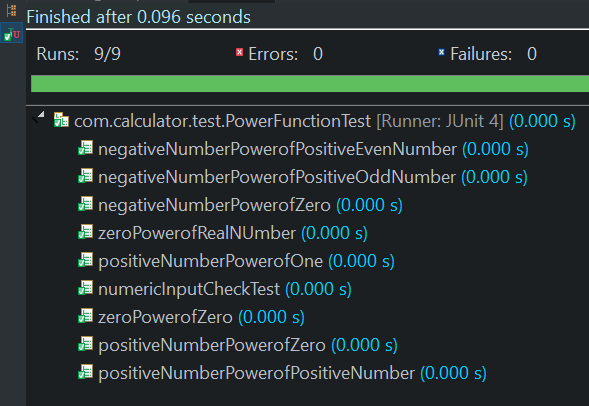
\includegraphics[width=13cm]{TestCases_Results_F7}
  \centering
  \caption{ Test case result of function F7 : \(x^y\)  using Junit4
}
\end{center}
\end{figure}
\end{document}